\documentclass[twoside]{book}

% Packages required by doxygen
\usepackage{fixltx2e}
\usepackage{calc}
\usepackage{doxygen}
\usepackage[export]{adjustbox} % also loads graphicx
\usepackage{graphicx}
\usepackage[utf8]{inputenc}
\usepackage{makeidx}
\usepackage{multicol}
\usepackage{multirow}
\PassOptionsToPackage{warn}{textcomp}
\usepackage{textcomp}
\usepackage[nointegrals]{wasysym}
\usepackage[table]{xcolor}

% Font selection
\usepackage[T1]{fontenc}
\usepackage[scaled=.90]{helvet}
\usepackage{courier}
\usepackage{amssymb}
\usepackage{sectsty}
\renewcommand{\familydefault}{\sfdefault}
\allsectionsfont{%
  \fontseries{bc}\selectfont%
  \color{darkgray}%
}
\renewcommand{\DoxyLabelFont}{%
  \fontseries{bc}\selectfont%
  \color{darkgray}%
}
\newcommand{\+}{\discretionary{\mbox{\scriptsize$\hookleftarrow$}}{}{}}

% Page & text layout
\usepackage{geometry}
\geometry{%
  a4paper,%
  top=2.5cm,%
  bottom=2.5cm,%
  left=2.5cm,%
  right=2.5cm%
}
\tolerance=750
\hfuzz=15pt
\hbadness=750
\setlength{\emergencystretch}{15pt}
\setlength{\parindent}{0cm}
\setlength{\parskip}{3ex plus 2ex minus 2ex}
\makeatletter
\renewcommand{\paragraph}{%
  \@startsection{paragraph}{4}{0ex}{-1.0ex}{1.0ex}{%
    \normalfont\normalsize\bfseries\SS@parafont%
  }%
}
\renewcommand{\subparagraph}{%
  \@startsection{subparagraph}{5}{0ex}{-1.0ex}{1.0ex}{%
    \normalfont\normalsize\bfseries\SS@subparafont%
  }%
}
\makeatother

% Headers & footers
\usepackage{fancyhdr}
\pagestyle{fancyplain}
\fancyhead[LE]{\fancyplain{}{\bfseries\thepage}}
\fancyhead[CE]{\fancyplain{}{}}
\fancyhead[RE]{\fancyplain{}{\bfseries\leftmark}}
\fancyhead[LO]{\fancyplain{}{\bfseries\rightmark}}
\fancyhead[CO]{\fancyplain{}{}}
\fancyhead[RO]{\fancyplain{}{\bfseries\thepage}}
\fancyfoot[LE]{\fancyplain{}{}}
\fancyfoot[CE]{\fancyplain{}{}}
\fancyfoot[RE]{\fancyplain{}{\bfseries\scriptsize Generated by Doxygen }}
\fancyfoot[LO]{\fancyplain{}{\bfseries\scriptsize Generated by Doxygen }}
\fancyfoot[CO]{\fancyplain{}{}}
\fancyfoot[RO]{\fancyplain{}{}}
\renewcommand{\footrulewidth}{0.4pt}
\renewcommand{\chaptermark}[1]{%
  \markboth{#1}{}%
}
\renewcommand{\sectionmark}[1]{%
  \markright{\thesection\ #1}%
}

% Indices & bibliography
\usepackage{natbib}
\usepackage[titles]{tocloft}
\setcounter{tocdepth}{3}
\setcounter{secnumdepth}{5}
\makeindex

% Hyperlinks (required, but should be loaded last)
\usepackage{ifpdf}
\ifpdf
  \usepackage[pdftex,pagebackref=true]{hyperref}
\else
  \usepackage[ps2pdf,pagebackref=true]{hyperref}
\fi
\hypersetup{%
  colorlinks=true,%
  linkcolor=blue,%
  citecolor=blue,%
  unicode%
}

% Custom commands
\newcommand{\clearemptydoublepage}{%
  \newpage{\pagestyle{empty}\cleardoublepage}%
}

\usepackage{caption}
\captionsetup{labelsep=space,justification=centering,font={bf},singlelinecheck=off,skip=4pt,position=top}

%===== C O N T E N T S =====

\begin{document}

% Titlepage & ToC
\hypersetup{pageanchor=false,
             bookmarksnumbered=true,
             pdfencoding=unicode
            }
\pagenumbering{roman}
\begin{titlepage}
\vspace*{7cm}
\begin{center}%
{\Large 41012 }\\
\vspace*{1cm}
{\large Generated by Doxygen 1.8.11}\\
\end{center}
\end{titlepage}
\clearemptydoublepage
\tableofcontents
\clearemptydoublepage
\pagenumbering{arabic}
\hypersetup{pageanchor=true}

%--- Begin generated contents ---
\chapter{A Sample for 41012 Students}
\label{index}\hypertarget{index}{}Our main goal is the continuing progress in robotic research and the robotic industry. The main challenge we see at present is the software specific to robots, both its complexity and the sheer amount of it.\hypertarget{index_ac_doc_index_more_info}{}\section{Where to start}\label{index_ac_doc_index_more_info}

\begin{DoxyItemize}
\item This just divides the general instructions here for students
\end{DoxyItemize}\hypertarget{index_ac_doc_install}{}\section{Installation}\label{index_ac_doc_install}
\hypertarget{index_ac_doc_step1}{}\subsection{Step 1\+: Opening the box}\label{index_ac_doc_step1}
Openning the box\hypertarget{index_ac_doc_step2}{}\subsection{Step 2\+: Running applications}\label{index_ac_doc_step2}
The system needs three components running, please run\+:

\begin{DoxyVerb}./tests/controller_test ../cfg/sim.cfg
./tests/lo_up ../cfg/sim.cfg
./tests/acLoc ../cfg/sim.cfg\end{DoxyVerb}
 
\chapter{Bug List}
\label{bug}
\hypertarget{bug}{}

\begin{DoxyRefList}
\item[\label{bug__bug000001}%
\hypertarget{bug__bug000001}{}%
Class \hyperlink{classShape}{Shape} ]none reported as of 2016-\/04-\/11 
\end{DoxyRefList}
\chapter{Hierarchical Index}
\section{Class Hierarchy}
This inheritance list is sorted roughly, but not completely, alphabetically\+:\begin{DoxyCompactList}
\item \contentsline{section}{Shape}{\pageref{classShape}}{}
\begin{DoxyCompactList}
\item \contentsline{section}{Rectangle}{\pageref{classRectangle}}{}
\end{DoxyCompactList}
\end{DoxyCompactList}

\chapter{Class Index}
\section{Class List}
Here are the classes, structs, unions and interfaces with brief descriptions\+:\begin{DoxyCompactList}
\item\contentsline{section}{\hyperlink{classRectangle}{Rectangle} }{\pageref{classRectangle}}{}
\item\contentsline{section}{\hyperlink{classShape}{Shape} \\*\hyperlink{classShape}{Shape} base class }{\pageref{classShape}}{}
\end{DoxyCompactList}

\chapter{Class Documentation}
\hypertarget{classRectangle}{}\section{Rectangle Class Reference}
\label{classRectangle}\index{Rectangle@{Rectangle}}
Inheritance diagram for Rectangle\+:\begin{figure}[H]
\begin{center}
\leavevmode
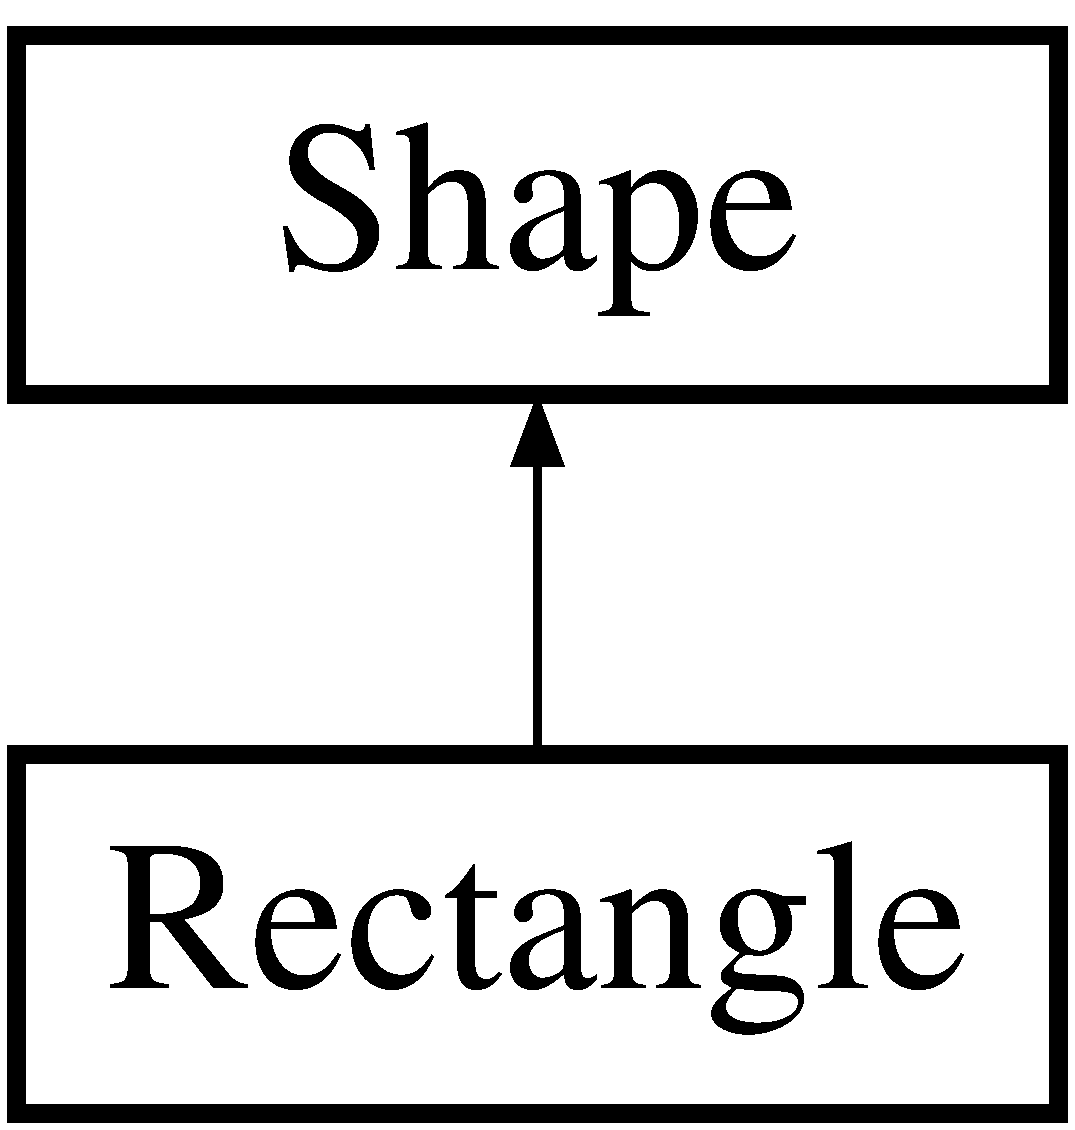
\includegraphics[height=2.000000cm]{classRectangle}
\end{center}
\end{figure}
\subsection*{Public Member Functions}
\begin{DoxyCompactItemize}
\item 
void \hyperlink{classRectangle_acf53f96f97e49fef43194574fd6dcaf0}{set\+Values} (double width, double height)
\item 
void {\bfseries set\+Values} (double side)\hypertarget{classRectangle_a4755ef0d81d47083e788a04e26271e08}{}\label{classRectangle_a4755ef0d81d47083e788a04e26271e08}

\item 
double \hyperlink{classRectangle_a953aa806e271319d14d18a3b473822a0}{get\+Area} (void)
\item 
double {\bfseries get\+Perimeter} (void)\hypertarget{classRectangle_a87d0d03c96128828d05d1b672ef83640}{}\label{classRectangle_a87d0d03c96128828d05d1b672ef83640}

\end{DoxyCompactItemize}
\subsection*{Additional Inherited Members}


\subsection{Member Function Documentation}
\index{Rectangle@{Rectangle}!get\+Area@{get\+Area}}
\index{get\+Area@{get\+Area}!Rectangle@{Rectangle}}
\subsubsection[{\texorpdfstring{get\+Area(void)}{getArea(void)}}]{\setlength{\rightskip}{0pt plus 5cm}double Rectangle\+::get\+Area (
\begin{DoxyParamCaption}
\item[{void}]{}
\end{DoxyParamCaption}
)}\hypertarget{classRectangle_a953aa806e271319d14d18a3b473822a0}{}\label{classRectangle_a953aa806e271319d14d18a3b473822a0}
This function returns the area of \hyperlink{classRectangle}{Rectangle} 
\begin{DoxyParams}[1]{Parameters}
\mbox{\tt out}  & {\em area} & of rectangle \\
\hline
\end{DoxyParams}
\index{Rectangle@{Rectangle}!set\+Values@{set\+Values}}
\index{set\+Values@{set\+Values}!Rectangle@{Rectangle}}
\subsubsection[{\texorpdfstring{set\+Values(double width, double height)}{setValues(double width, double height)}}]{\setlength{\rightskip}{0pt plus 5cm}void Rectangle\+::set\+Values (
\begin{DoxyParamCaption}
\item[{double}]{width, }
\item[{double}]{height}
\end{DoxyParamCaption}
)}\hypertarget{classRectangle_acf53f96f97e49fef43194574fd6dcaf0}{}\label{classRectangle_acf53f96f97e49fef43194574fd6dcaf0}
This function sets the width and height of a \hyperlink{classRectangle}{Rectangle}


\begin{DoxyParams}[1]{Parameters}
\mbox{\tt in}  & {\em width} & dimension of rectangle \\
\hline
\mbox{\tt in}  & {\em height} & dimension of rectangke \\
\hline
\end{DoxyParams}


The documentation for this class was generated from the following files\+:\begin{DoxyCompactItemize}
\item 
/home/user/git/pfms-\/2020a-\/esteban-\/andrade/scratch/week04/starter/doxygen\+\_\+example/rectangle.\+h\item 
/home/user/git/pfms-\/2020a-\/esteban-\/andrade/scratch/week04/starter/doxygen\+\_\+example/rectangle.\+cpp\end{DoxyCompactItemize}

\hypertarget{classShape}{}\section{Shape Class Reference}
\label{classShape}\index{Shape@{Shape}}


\hyperlink{classShape}{Shape} base class.  




{\ttfamily \#include $<$shape.\+h$>$}

Inheritance diagram for Shape\+:\begin{figure}[H]
\begin{center}
\leavevmode
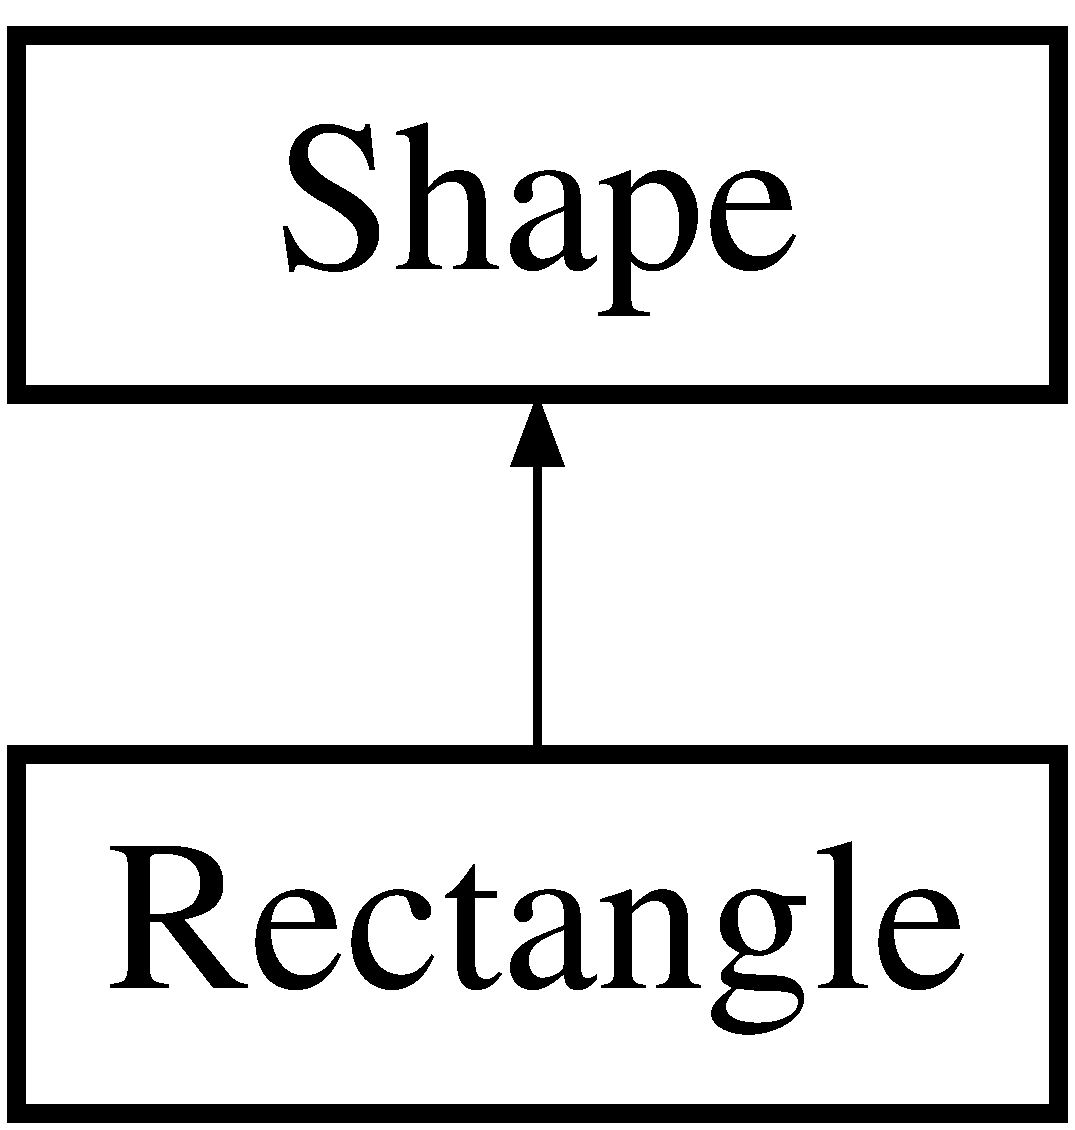
\includegraphics[height=2.000000cm]{classShape}
\end{center}
\end{figure}
\subsection*{Public Member Functions}
\begin{DoxyCompactItemize}
\item 
double \hyperlink{classShape_a979c49fdf29dde347a2e83f779ca78bd}{get\+Area} (void)
\begin{DoxyCompactList}\small\item\em Computes the area and returns value \mbox{[}m2\mbox{]}. \end{DoxyCompactList}\item 
double {\bfseries get\+Perimeter} (void)\hypertarget{classShape_aeaeb4227da008cd7491691b2f3d89292}{}\label{classShape_aeaeb4227da008cd7491691b2f3d89292}

\item 
std\+::string {\bfseries get\+Description} ()\hypertarget{classShape_a8bedf1ca522a2d0280a52d819cb55bf8}{}\label{classShape_a8bedf1ca522a2d0280a52d819cb55bf8}

\end{DoxyCompactItemize}
\subsection*{Protected Attributes}
\begin{DoxyCompactItemize}
\item 
std\+::string \hyperlink{classShape_a67e9566e302b377f2a6d2032fdad48e2}{description\+\_\+}\hypertarget{classShape_a67e9566e302b377f2a6d2032fdad48e2}{}\label{classShape_a67e9566e302b377f2a6d2032fdad48e2}

\begin{DoxyCompactList}\small\item\em description of shape \end{DoxyCompactList}\end{DoxyCompactItemize}


\subsection{Detailed Description}
\hyperlink{classShape}{Shape} base class. 

This class is the base class for all shapes.~\newline
\begin{DoxyAuthor}{Author}
Alen Alempijevic 

Alex Virgona 
\end{DoxyAuthor}
\begin{DoxyVersion}{Version}
1.\+02-\/1 
\end{DoxyVersion}
\begin{DoxyDate}{Date}
2016 
\end{DoxyDate}
\begin{DoxyPrecond}{Precondition}
none 
\end{DoxyPrecond}
\begin{DoxyRefDesc}{Bug}
\item[\hyperlink{bug__bug000001}{Bug}]none reported as of 2016-\/04-\/11 \end{DoxyRefDesc}
\begin{DoxyWarning}{Warning}

\end{DoxyWarning}


\subsection{Member Function Documentation}
\index{Shape@{Shape}!get\+Area@{get\+Area}}
\index{get\+Area@{get\+Area}!Shape@{Shape}}
\subsubsection[{\texorpdfstring{get\+Area(void)}{getArea(void)}}]{\setlength{\rightskip}{0pt plus 5cm}double Shape\+::get\+Area (
\begin{DoxyParamCaption}
\item[{void}]{}
\end{DoxyParamCaption}
)}\hypertarget{classShape_a979c49fdf29dde347a2e83f779ca78bd}{}\label{classShape_a979c49fdf29dde347a2e83f779ca78bd}


Computes the area and returns value \mbox{[}m2\mbox{]}. 

\begin{DoxyReturn}{Returns}
The area 
\end{DoxyReturn}
\begin{DoxySeeAlso}{See also}
\hyperlink{classShape}{Shape()} and get\+Description() 
\end{DoxySeeAlso}


The documentation for this class was generated from the following files\+:\begin{DoxyCompactItemize}
\item 
/home/user/git/pfms-\/2020a-\/esteban-\/andrade/scratch/week04/starter/doxygen\+\_\+example/shape.\+h\item 
/home/user/git/pfms-\/2020a-\/esteban-\/andrade/scratch/week04/starter/doxygen\+\_\+example/shape.\+cpp\end{DoxyCompactItemize}

%--- End generated contents ---

% Index
\backmatter
\newpage
\phantomsection
\clearemptydoublepage
\addcontentsline{toc}{chapter}{Index}
\printindex

\end{document}
